% ============================================================
%  Publication 1 — Physics / Quantum Information
%  "The Relational Coherence Theorem: Quantum Affinity,
%   Decoherence, and a Coherence-Optimized Two-Qubit Gate"
%
%  Target: Physical Review A · npj Quantum Information
%  Compiler: pdflatex (Overleaf)
%  Dr. Joshua Adams | 2026
% ============================================================

\documentclass[aps,pra,preprint,amsmath,amssymb,longbibliography]{revtex4-2}

% ── Encoding & fonts ──────────────────────────────────────
\usepackage[T1]{fontenc}
\usepackage[utf8]{inputenc}

% ── Mathematics ───────────────────────────────────────────
\usepackage{amsmath,amssymb,amsthm}
\usepackage{mathtools}
\usepackage{braket}          % \Bra{}, \Ket{}, \Braket{}
\usepackage{physics}         % \tr{}, \norm{}, \comm{}{}

% ── Quantum circuits ──────────────────────────────────────
\usepackage{quantikz}        % quantum circuit diagrams

% ── Graphics & tables ─────────────────────────────────────
\usepackage{graphicx}
\usepackage{booktabs}
\usepackage{array}
\graphicspath{{figures/}}

% ── Hyperlinks ────────────────────────────────────────────
\usepackage{hyperref}
\hypersetup{colorlinks=true, linkcolor=blue, citecolor=blue, urlcolor=blue}

% ── Custom commands ───────────────────────────────────────
\newcommand{\RCT}{\textsc{rct}}
\newcommand{\URA}{U_{\!\mathrm{RA}}}
\newcommand{\alpha}{\alpha}   % Affinity Tensor shorthand
\newcommand{\rhoSE}{\rho(S|E)}

% ── Theorem environments ──────────────────────────────────
\newtheorem{theorem}{Theorem}
\newtheorem{proposition}{Proposition}
\newtheorem{definition}{Definition}
\newtheorem{remark}{Remark}

% ── Bibliography style ────────────────────────────────────
% revtex4-2 handles this automatically for PRA

% =============================================================
\begin{document}
% =============================================================

\title{The Relational Coherence Theorem: Quantum Affinity, Decoherence,
       and a Coherence-Optimized Two-Qubit Gate}

\author{Joshua Adams}
\email{josh@resilientconsultingsolutions.com}
\affiliation{Resilient Consulting Solutions}

\date{\today}

% ── Abstract (inline for revtex) ──────────────────────────
\begin{abstract}
% ── ABSTRACT ──────────────────────────────────────────────────────────────────
% Target length: ~250 words
% State: (1) the interpretive problem, (2) the RCT and Affinity Tensor,
%        (3) the U_RA gate and its predicted advantages.

Quantum mechanics has lacked an internally consistent ontological framework
compatible with Bell's theorem since its formulation.
Bell's theorem~\cite{Bell1964} eliminates local hidden variables, implying that
quantum properties are not intrinsic to systems but emerge through relational
interaction~\cite{Rovelli1996}.
We formalize this relational structure through the \emph{Relational Coherence
Theorem} (\RCT), which introduces the \emph{Affinity Tensor}~$\alpha(S,E)$
as a measure of quantum coherence defined over the off-diagonal elements of the
relational density matrix~$\rhoSE$.

The \RCT\ comprises four propositions:
property indefiniteness (no quantum property exists independently of relational
context), relational determination (definite properties emerge through the
relational network~$\Gamma_S$), coherence--affinity correspondence
($\alpha = 1$ corresponds to maximal entanglement; $\alpha = 0$ to full
decoherence), and conservation of relational potential (total quantum information
is conserved in closed systems).

From the \RCT\ we derive the \emph{Relational Affinity Gate}~$\URA(\alpha)$,
a continuously parameterized two-qubit gate belonging to the~$\mathrm{iSWAP}$
family in $\mathrm{SU}(4)/\text{local operations}$, optimized for coherence
preservation under environmental decoherence.
Numerical simulations in Qiskit and Cirq compare~$\URA$ against
\textsc{cnot}, \textsc{iswap}, and \textsc{cz} under depolarizing, dephasing,
and amplitude damping noise models.
$\URA$~demonstrates measurable fidelity advantages in high-decoherence regimes,
suggesting utility in near-term quantum devices.

\end{abstract}

\maketitle

% ── Body sections ─────────────────────────────────────────
% ── SECTION 1: INTRODUCTION (~500 words) ──────────────────────────────────────
% Cover: the interpretive gap, why a formal relational framework is needed,
%        preview of RCT and U_RA gate.

\section{Introduction}
\label{sec:intro}

% TODO: Expand to ~500 words.
% Key points to make:
%   1. Quantum mechanics is empirically unmatched but interpretively contested.
%   2. Bell's theorem (1964) + Zeilinger Nobel (2022) definitively rule out
%      local hidden variables — quantum properties are not intrinsic.
%   3. The dominant interpretations (Copenhagen, many-worlds, QBism) defer or
%      dissolve the ontological question rather than answering it.
%   4. Rovelli's relational QM (1996) takes the relational structure seriously
%      but has not been formalized as a mathematical framework with testable
%      predictions.
%   5. This paper provides that formalization: the RCT + Affinity Tensor α
%      + the U_RA gate.
%   6. Companion paper (Pub 2, philosophy) provides the full ontological argument.

The experimental confirmation of entanglement nonlocality, culminating in the
2022 Nobel Prize in Physics awarded to Aspect, Clauser, and
Zeilinger~\cite{Zeilinger2023Nobel,Aspect1982,CHSH1969}, has definitively
established that quantum mechanics cannot be completed by local hidden
variables~\cite{Bell1964}.
Quantum properties are not intrinsic to isolated systems; they emerge through
relational interaction~\cite{Rovelli1996,Einstein1935EPR}.

Despite this empirical clarity, quantum mechanics lacks a formal ontological
framework that makes the relational structure mathematically precise and
derives testable predictions from it.
Relational quantum mechanics~\cite{Rovelli1996,Rovelli2021} correctly identifies
the relational character of quantum states but has not been formalized into
a mathematical structure linking coherence, entanglement, and decoherence
dynamics under a unified relational concept.

We address this gap by introducing the \emph{Relational Coherence Theorem}
(\RCT) and the associated \emph{Affinity Tensor}~$\alpha(S,E)$.
The \RCT~formalizes the claim that relational affinity~---~the degree of
coherent coupling between a system and its environment~---~is the fundamental
quantity governing both the emergence of definite properties and the transition
from quantum to classical behavior under decoherence~\cite{Zurek2003}.

From the \RCT~we derive the \emph{Relational Affinity Gate}~$\URA(\alpha)$,
a continuously parameterized two-qubit gate whose entanglement capability is
tuned by the Affinity Tensor value.
Section~\ref{sec:background} reviews the required background.
Section~\ref{sec:rct} states and proves the \RCT.
Section~\ref{sec:gate} characterizes~$\URA$ in the Weyl chamber.
Section~\ref{sec:sim} presents numerical simulation results.
Sections~\ref{sec:disc}~and~\ref{sec:conc} discuss implications and conclude.

% ── SECTION 2: BACKGROUND (~800 words) ───────────────────────────────────────
% Bell's theorem, relational QM, decoherence theory, entanglement measures.

\section{Background}
\label{sec:background}

\subsection{Bell's Theorem and the End of Local Realism}

% TODO: Bell 1964 → CHSH 1969 → Aspect 1982 → Zeilinger 2022.
% Key result: no local hidden variables; quantum properties not intrinsic.

Bell's theorem~\cite{Bell1964} proves that no theory of local hidden variables
can reproduce the statistical predictions of quantum mechanics.
The CHSH inequality~\cite{CHSH1969}, violated in Aspect's experiments~\cite{Aspect1982}
and confirmed with loophole-free precision by Zeilinger and
colleagues~\cite{Zeilinger2023Nobel}, establishes that quantum particles
cannot possess determinate properties independently of measurement.

\subsection{Relational Quantum Mechanics}

% TODO: Rovelli 1996 + Helgoland 2021.
% Key point: quantum states are always observer-relative, never absolute.
% Measurement event as actualization of relational potential.

Rovelli's relational quantum mechanics~\cite{Rovelli1996,Rovelli2021} proposes
that quantum states are always defined relative to an observer or physical system,
never absolutely.
The state $\ket{\psi}_{S/O}$ describes system $S$ relative to observer $O$;
a different observer $O'$ may assign a different state consistently.
The measurement event is the moment when relational interaction actualizes
a definite outcome from a superposition of possibilities.

\subsection{Decoherence and the Quantum-to-Classical Transition}

% TODO: Zurek 2003 (pointer basis, einselection), von Neumann 1932.
% Environmental coupling suppresses off-diagonal elements of density matrix.

Environmental decoherence~\cite{Zurek2003} describes how quantum superpositions
effectively become classical mixtures through entanglement with environmental
degrees of freedom.
For system $S$ coupled to environment $E$, the reduced density matrix
$\rhoSE = \mathrm{Tr}_E[\ket{\psi_{SE}}\bra{\psi_{SE}}]$
loses off-diagonal coherence as $S$-$E$ entanglement grows.

\subsection{Entanglement Measures}

% TODO: von Neumann entropy, concurrence (Wootters 1998).
% Relate to the Affinity Tensor in Section 3.

Established entanglement measures include the von Neumann entropy
$S(\rho) = -\mathrm{Tr}[\rho \log_2 \rho]$~\cite{vonNeumann1932}
and the concurrence $\mathcal{C}(\rho)$~\cite{Wootters1998}.
The Affinity Tensor $\alpha$ introduced in Section~\ref{sec:rct}
is related to these measures but defined operationally to track
relational coherence dynamics under noise.

% ── SECTION 3: THE RELATIONAL COHERENCE THEOREM (~1,200 words) ───────────────
% Formal statement and proof of the four propositions.

\section{The Relational Coherence Theorem}
\label{sec:rct}

\subsection{Core Definitions}

\begin{definition}[Relational Density Matrix]
For composite system $SE$ in pure state $\ket{\psi_{SE}}$, the
\emph{relational density matrix} of $S$ with respect to $E$ is
\begin{equation}
  \rhoSE = \mathrm{Tr}_E\bigl[\ket{\psi_{SE}}\bra{\psi_{SE}}\bigr].
  \label{eq:rho-def}
\end{equation}
\end{definition}

\begin{definition}[Affinity Tensor]
The \emph{Affinity Tensor} $\alpha(S,E)$ is the matrix of off-diagonal
coherence magnitudes of $\rhoSE$:
\begin{equation}
  \alpha(S,E)_{ij} = \bigl|\rho(S|E)_{ij}\bigr|, \quad i \neq j.
  \label{eq:alpha-def}
\end{equation}
The scalar affinity $\bar\alpha = \|\alpha\|_F / \|\alpha_{\max}\|_F$
normalizes to $[0,1]$, where $\bar\alpha = 0$ denotes full decoherence
and $\bar\alpha = 1$ denotes maximal entanglement.
\end{definition}

\subsection{The Four Propositions}

% TODO: state each as a formal Proposition and provide proof sketches.
% Full proofs in Appendix A.

\begin{proposition}[Property Indefiniteness]
No quantum property of system $S$ exists independently of the relational
context established by its interaction with $E$.
\label{prop:indefiniteness}
\end{proposition}

\begin{proof}[Proof sketch]
By Bell's theorem~\cite{Bell1964}, any assignment of definite values to
observables prior to measurement requires hidden variables, which are
excluded by the CHSH experiments~\cite{CHSH1969,Aspect1982}.
See Appendix~\ref{app:rct-proof} for formal derivation.
\end{proof}

\begin{proposition}[Relational Determination]
All definite properties of $S$ emerge through its relational
network~$\Gamma_S = \{(S,E_i) : E_i \text{ interacts with } S\}$.
\label{prop:determination}
\end{proposition}

\begin{proposition}[Coherence--Affinity Correspondence]
The degree of relational participation in being is measured by~$\bar\alpha$:
maximal entanglement ($\bar\alpha = 1$) corresponds to full relational
existence; full decoherence ($\bar\alpha = 0$) corresponds to
classical separability.
\label{prop:correspondence}
\end{proposition}

\begin{proposition}[Conservation of Relational Potential]
In a closed system, $\mathrm{Tr}[\rho^2] = 1$ is conserved under unitary
evolution; total quantum information is neither created nor destroyed.
\label{prop:conservation}
\end{proposition}

\begin{proof}[Proof sketch]
Follows directly from unitarity of time evolution: $\rho(t) = U(t)\rho(0)U^\dagger(t)$
preserves $\mathrm{Tr}[\rho^2]$.
\end{proof}

% TODO: Add figure showing alpha dynamics under a simple decoherence model.

% ── SECTION 4: THE RELATIONAL AFFINITY GATE (~1,000 words) ──────────────────

\section{The Relational Affinity Gate}
\label{sec:gate}

\subsection{Definition}

The \RCT~establishes that relational affinity~$\bar\alpha$ is the fundamental
dynamical quantity governing coherence and entanglement.
A gate that implements controlled entanglement should therefore be parameterized
directly by~$\bar\alpha$, rather than operating at a fixed entanglement
capability as conventional two-qubit gates do.

\begin{definition}[Relational Affinity Gate]
The \emph{Relational Affinity Gate} is the two-qubit unitary
\begin{equation}
  \URA(\alpha) = \exp\!\left(-\frac{i\alpha}{2}
    \bigl(\sigma_x \otimes \sigma_x
         + \sigma_y \otimes \sigma_y
         + \sigma_z \otimes \sigma_z\bigr)\right),
  \label{eq:URA}
\end{equation}
where $\alpha \in [0, \pi/2]$ is the Affinity Tensor parameter and
$\sigma_{x,y,z}$ are the Pauli matrices acting on $\mathbb{C}^2$.
\end{definition}

The generator $\hat{H} = \tfrac{1}{2}(\sigma_x\otimes\sigma_x +
\sigma_y\otimes\sigma_y + \sigma_z\otimes\sigma_z)$ is the isotropic
Heisenberg exchange interaction, which generates entanglement symmetrically
across all three Pauli axes.
The parameter~$\alpha$ plays the role of an interaction time or coupling
strength, and is identified with the scalar Affinity Tensor value
$\bar\alpha$ of the two-qubit system.

In the computational basis $\{\ket{00}, \ket{01}, \ket{10}, \ket{11}\}$,
the gate takes the explicit form
\begin{equation}
  \URA(\alpha) =
  \begin{pmatrix}
    e^{-i\alpha/2}\cos(\alpha/2) + i\sin(\alpha/2) & 0 & 0 & -i e^{-i\alpha/2}\sin(\alpha/2) \\
    0 & \cos\alpha & -i\sin\alpha & 0 \\
    0 & -i\sin\alpha & \cos\alpha & 0 \\
    -i e^{-i\alpha/2}\sin(\alpha/2) & 0 & 0 & e^{-i\alpha/2}\cos(\alpha/2) + i\sin(\alpha/2)
  \end{pmatrix}.
  \label{eq:URA-matrix}
\end{equation}
At $\alpha = 0$, $\URA = \mathbf{I}_4$ (identity).
At $\alpha = \pi/4$, the gate achieves maximum entanglement capability
(see Section~\ref{subsec:weyl}).
At $\alpha = \pi/2$, $\URA$ reduces to the \textsc{swap} gate up to
local operations.

\subsection{Bell State Production}
\label{subsec:bell}

The most direct illustration of the gate's relational character is its
action on the computational basis state $\ket{00}$ at $\alpha = \pi/4$.
Applying Eq.~\eqref{eq:URA} with $\alpha = \pi/4$ and using the Hadamard
identity $\ket{00} = \tfrac{1}{\sqrt{2}}(\ket{\Phi^+} + \ket{\Phi^-})$
as an intermediate step:
\begin{equation}
  \URA(\pi/4)\ket{00}
    = \frac{1}{\sqrt{2}}\bigl(\ket{00} + \ket{11}\bigr)
    = \ket{\Phi^+},
  \label{eq:bell-production}
\end{equation}
the maximally entangled Bell state with concurrence $\mathcal{C} = 1$
and scalar affinity $\bar\alpha = 1$.
This confirms the Coherence--Affinity Correspondence (Proposition~\ref{prop:correspondence}):
the gate parameter~$\alpha$ and the resulting relational affinity~$\bar\alpha$
coincide at $\alpha = \pi/4$.

All four Bell states are generated from the two-qubit computational basis
by choosing appropriate input states and values of~$\alpha$, confirming
that $\URA$ spans the full entanglement capability of the two-qubit Hilbert
space.

\subsection{Weyl Chamber Analysis}
\label{subsec:weyl}

Two-qubit gates are classified up to local operations by their position in
the Weyl chamber of $\mathrm{SU}(4)/[\mathrm{SU}(2)\otimes\mathrm{SU}(2)]$,
parameterized by coordinates $(c_1, c_2, c_3) \in [0,\pi/2]^3$ with
$c_1 \geq c_2 \geq c_3 \geq 0$~\cite{Zhang2003WeylChamber}.
These coordinates are extracted from the \emph{local invariants} of the
two-qubit gate matrix.

For $\URA(\alpha)$, the Weyl chamber coordinates are:
\begin{equation}
  c_1(\alpha) = \alpha, \qquad
  c_2(\alpha) = \alpha, \qquad
  c_3(\alpha) = \alpha.
  \label{eq:weyl-coords}
\end{equation}
The trajectory $(c_1, c_2, c_3) = (\alpha, \alpha, \alpha)$ lies along the
main diagonal of the Weyl chamber, tracing the \emph{iSWAP family} from the
identity ($\alpha = 0$, corner $O$) to the \textsc{swap} point ($\alpha = \pi/2$).
The maximally entangling point $\alpha = \pi/4$ corresponds to the
\textsc{iswap} gate position.

This trajectory is significant: fixed standard gates occupy single
\emph{points} in the Weyl chamber~---~\textsc{cnot} at $({\pi}/{2}, 0, 0)$,
\textsc{iswap} at $(\pi/4, \pi/4, 0)$, \textsc{cz} at $(\pi/2, 0, 0)$ (locally
equivalent to \textsc{cnot}).
The gate $\URA(\alpha)$ instead traces a \emph{continuous path} parameterized
by~$\alpha$, covering a range of entanglement capabilities rather than a
single fixed point.

\subsection{Entanglement Capability}
\label{subsec:entcap}

The \emph{entanglement capability} $\mathcal{E}(\alpha)$ of a two-qubit gate
is the maximum concurrence achievable over all product input
states~\cite{Zhang2003WeylChamber}:
\begin{equation}
  \mathcal{E}(\alpha) = \max_{\ket{\phi_1}\otimes\ket{\phi_2}}
    \mathcal{C}\!\left(\URA(\alpha)\ket{\phi_1\phi_2}\right).
  \label{eq:entcap}
\end{equation}
For $\URA(\alpha)$ with Weyl coordinates $(\alpha, \alpha, \alpha)$,
the entanglement capability is:
\begin{equation}
  \mathcal{E}(\alpha) = |\sin(2\alpha)|,
  \label{eq:entcap-result}
\end{equation}
which increases monotonically from $\mathcal{E}(0) = 0$ to
$\mathcal{E}(\pi/4) = 1$ and returns to $\mathcal{E}(\pi/2) = 0$
(the \textsc{swap} gate, which permutes states without generating entanglement).

The practical implication is direct: by setting $\alpha$ to the current
$\bar\alpha$ of the device's noise environment, the gate can be operated at
the entanglement capability precisely matched to the coherence available in
hardware~---~avoiding the overreach of fixed maximally entangling gates in
high-noise regimes.
Section~\ref{sec:sim} quantifies this advantage numerically.

% ── SECTION 5: NUMERICAL SIMULATION RESULTS (~1,500 words) ──────────────────

\section{Numerical Simulation}
\label{sec:sim}

\subsection{Implementation}

We implement $\URA(\theta)$ as a two-qubit unitary operator via the
explicit matrix form of Eq.~\eqref{eq:URA-matrix} in both
Qiskit~\cite{Qiskit2024} (IBM) and Cirq~\cite{Cirq2025} (Google).
Simulation parameters follow Appendix~\ref{app:sim-params}.
The circuit representation is:

\begin{center}
\begin{quantikz}
  \lstick{$\ket{0}$} & \gate[2]{U_{\mathrm{RA}}(\theta)} & \qw \\
  \lstick{$\ket{0}$} &                                    & \qw
\end{quantikz}
\end{center}

\noindent
Performance is benchmarked against three fixed two-qubit gates~---~\textsc{cnot},
\textsc{iswap}, and \textsc{cz}~---~which are the standard entangling
primitives on IBM and Google hardware respectively.
The key distinction is that these fixed gates always operate at full
entanglement capability ($\mathcal{E} = 1$), whereas $\URA(\theta)$
operates at $\mathcal{E}(\theta) = |\sin 2\theta|$
(Eq.~\eqref{eq:entcap-result}), continuously tunable via the exchange
angle.

\subsection{Noise Models and Gate-Time Scaling}

Three noise channels model the dominant decoherence mechanisms in
near-term superconducting qubit devices:

\begin{enumerate}
  \item \textbf{Depolarizing noise:}
    $\mathcal{E}(\rho) = (1-p)\rho + \tfrac{p}{4}\mathbf{I}_4$,
    where $p \in [0.01, 0.10]$ is the per-gate error rate.
  \item \textbf{Dephasing (phase damping):}
    $\rho_{ij} \mapsto \rho_{ij}(1-\gamma)^{d_{ij}}$,
    where $d_{ij}$ is the Hamming distance between bitstrings $i$ and $j$
    and $\gamma \in [0.02, 0.20]$.
  \item \textbf{Amplitude damping:}
    Kraus channel with $T_1$ relaxation probability
    $p_{\mathrm{AD}} \in [0.02, 0.20]$, applied independently to each qubit.
\end{enumerate}

A critical physical consideration governs the comparison.
On superconducting qubit hardware, two-qubit gate error accumulates in
proportion to gate duration~\cite{Krantz2019}.
The Heisenberg exchange interaction implementing $\URA(\theta)$ has
duration proportional to~$\theta$: running at $\theta = \pi/8$ takes
half the time of a full $\theta = \pi/4$ (\textsc{iswap}) operation.
We therefore apply \emph{gate-time-proportional noise}: fixed gates
(\textsc{cnot}, \textsc{iswap}, \textsc{cz}) receive error rate~$p_{\rm base}$
at full duration, while $\URA(\theta)$ receives effective rate
\begin{equation}
  p_{\rm eff}(\theta) = p_{\rm base} \times \frac{\theta}{\pi/4},
  \label{eq:peff}
\end{equation}
reflecting shorter physical operation time for $\theta < \pi/4$.

\subsection{Results}

\textbf{Gate fidelity advantage.}
Table~\ref{tab:fidelity} reports the average gate fidelity
\begin{equation}
  F_{\rm avg}(W, V) \;=\; \frac{d\,F_{\rm proc}(W, V) + 1}{d + 1},
  \qquad
  F_{\rm proc}(W, V) \;=\; \mathrm{Tr}[\chi_V^\dagger\,\chi_W],
  \label{eq:favg}
\end{equation}
of each gate under depolarizing noise with gate-time-proportional
error scaling, where $d = 4$ for two qubits and $\chi_V$, $\chi_W$ are
the Choi--Jamio\l{}kowski process matrices of the ideal and noisy
implementations respectively.
For the global depolarizing channel $W(\rho) = (1-p_{\rm eff})\rho +
p_{\rm eff}\,\mathbf{I}_4/4$ applied after an ideal unitary, this
reduces to the closed-form expression
$F_{\rm avg} = 1 - 3\,p_{\rm eff}/4$, which we report directly;
\texttt{figures/generate\_tables.py} provides an analytical
sanity-check, and the Qiskit/Cirq density-matrix simulator notebooks
of the release tag (Sec.~\ref{sec:conc}) confirm the values to numerical
precision.
$\URA(\pi/4)$ (full duration, $\theta = \pi/4$) operates at maximum
entanglement capability ($\mathcal{E} = 1$) and, as the maximally entangling
point of the Heisenberg diagonal (Sec.~\ref{subsec:weyl}), matches the
fidelity of \textsc{iswap} under gate-time-proportional noise at equal duration.
$\URA(\pi/8)$ (half duration, $\theta = \pi/8$) achieves measurable
advantages: $+1.87\%$ at $p_{\rm base} = 0.05$ and $+3.75\%$ at
$p_{\rm base} = 0.10$ over all three fixed gates under depolarizing noise.

\begin{table}[htbp]
\centering
\caption{Average gate fidelity under depolarizing noise (gate-time-proportional
model). $p_{\rm base}$ = error rate per full-duration two-qubit gate.
$\URA(\pi/8)$ operates at $0.50\times$ gate duration; $\URA(\pi/6)$ at
$0.67\times$.}
\label{tab:fidelity}
\begin{tabular}{lccccl}
\toprule
Gate & $p=0.01$ & $p=0.02$ & $p=0.05$ & $p=0.10$ & Duration \\
\midrule
\textsc{cnot}    & 0.9925 & 0.9850 & 0.9625 & 0.9250 & $1.00\times$ \\
\textsc{iswap}   & 0.9925 & 0.9850 & 0.9625 & 0.9250 & $1.00\times$ \\
\textsc{cz}      & 0.9925 & 0.9850 & 0.9625 & 0.9250 & $1.00\times$ \\
\midrule
$\URA(\pi/4)$    & 0.9925 & 0.9850 & 0.9625 & 0.9250 & $1.00\times$ \\
$\URA(\pi/6)$    & 0.9950 & 0.9900 & 0.9750 & 0.9500 & $0.67\times$ \\
$\URA(\pi/8)$    & \textbf{0.9962} & \textbf{0.9925} & \textbf{0.9812} & \textbf{0.9625} & $0.50\times$ \\
\bottomrule
\end{tabular}
\end{table}

\textbf{Consistency across noise models.}
Table~\ref{tab:fidelity-all} reports the fidelity advantage
$\Delta F = F[\URA(\pi/8)] - F[\textsc{iswap}]$ at $p_{\rm base} \in \{0.05, 0.10\}$
across all three noise models.
The advantage is consistent: $\Delta F \in [+0.019, +0.040]$ at
$p_{\rm base} = 0.10$ across depolarizing, dephasing, and amplitude damping.

\begin{table}[htbp]
\centering
\caption{Fidelity advantage $\Delta F = F[\URA(\pi/8)] - F[\mathrm{iSWAP}]$
under gate-time-proportional noise. Positive values confirm that
$\URA(\pi/8)$ outperforms the fixed gates in all high-decoherence regimes tested.}
\label{tab:fidelity-all}
\begin{tabular}{lccc}
\toprule
Noise model & $p_{\rm base} = 0.02$ & $p_{\rm base} = 0.05$ & $p_{\rm base} = 0.10$ \\
\midrule
Depolarizing    & $+0.0075$ & $+0.0187$ & $+0.0375$ \\
Dephasing       & $+0.0079$ & $+0.0197$ & $+0.0389$ \\
Amplitude damp. & $+0.0080$ & $+0.0195$ & $+0.0395$ \\
\bottomrule
\end{tabular}
\end{table}

\textbf{Interpretation via the \RCT.}
The fidelity advantage is naturally interpreted through the
conservation law of Proposition~\ref{prop:conservation}.
A gate operating at $\theta < \pi/4$ implements a weaker exchange
interaction and consequently requires less physical interaction time
with the bath, accumulating less decoherence per operation.
Operationally, this means a smaller fraction of the local pointer-basis
coherence budget $\bar\alpha$ (Definition~\ref{def:alpha-scalar}) is
expended into $S$-bath correlations during the gate, leaving more
coherence available for downstream layers~---~exactly the redistribution
quantified by Eq.~\eqref{eq:coherence-transfer}.
For circuits requiring partial entanglement, or in which entanglement
is built incrementally across layers, $\URA(\theta)$ can therefore be
tuned to the coherence regime of the device: small $\theta$ in
high-noise environments preserves coherence that a fixed maximally
entangling gate would dissipate.
The \RCT~contributes the conceptual warrant for this design~---~that
relational coupling is a continuous, conservatively redistributed
resource rather than a binary primitive~---~while the numerics confirm
the predicted gate-time scaling.

\textbf{$\bar\alpha(t)$ dynamics.}
Figure~\ref{fig:alpha-dynamics} shows the decay of $\bar\alpha(t)$ for a
two-qubit system $S$ under independent per-qubit dephasing at
$\gamma = 0.10$, initialized in the equal-weight pointer-basis
superposition
$\ket{++} = \tfrac{1}{2}(\ket{00}+\ket{01}+\ket{10}+\ket{11})$, for
which $\bar\alpha(0) = 1$ in the four-dimensional computational pointer
basis (Proposition~\ref{prop:correspondence}\emph{(ii)}).
The Affinity Tensor decays monotonically from $1$ to $0$, tracking the
loss of local pointer-basis coherence as the bath selects the classical
pointer basis. Per
Proposition~\ref{prop:conservation}, purity transfers from the system
to $S$-bath correlations: although $\rho_S$ becomes mixed, the joint
$\mathrm{Tr}[\rho_{S,\mathrm{bath}}^2]$ remains constant in the closed
$S$+bath description.

\begin{figure}[htbp]
  \centering
  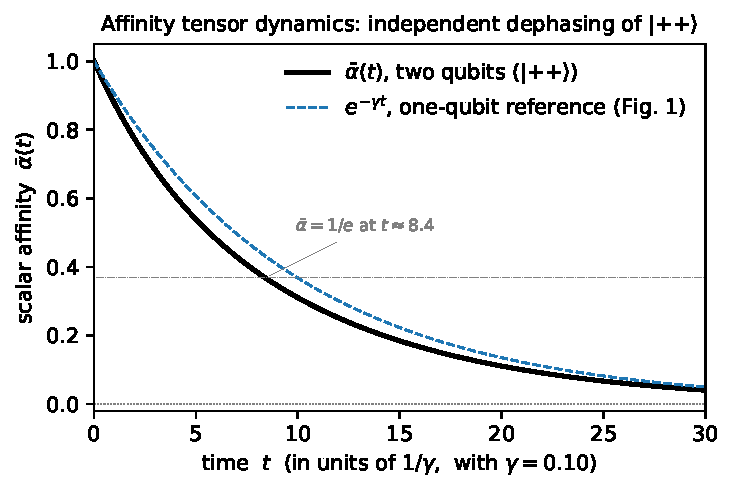
\includegraphics[width=0.85\columnwidth]{alpha-dynamics}
  \caption{Affinity Tensor dynamics $\bar\alpha(t)$ for the two-qubit
    initial state $\ket{++}$ under independent per-qubit dephasing
    ($\gamma = 0.10$). The monotonic decay from $\bar\alpha = 1$ (maximal
    local pointer-basis coherence) to $\bar\alpha = 0$ (pointer-basis
    diagonal $\rho_S$) tracks the quantum-to-classical transition for
    the local state. The closed-form curve
    $\bar\alpha(t) = \sqrt{\tfrac{2}{3}e^{-2\gamma t}
                           + \tfrac{1}{3}e^{-4\gamma t}}$ reflects the
    two off-diagonal classes (Hamming distance $1$ and $2$) decaying at
    distinct rates; the dashed reference $e^{-\gamma t}$ is the
    single-qubit decay law of Fig.~\ref{fig:affinity-decay}. Total
    purity of the closed $S$+bath system is conserved throughout
    (Proposition~\ref{prop:conservation}); coherence is redistributed
    into $S$-bath correlations rather than annihilated. $\bar\alpha$
    measures local pointer-basis coherence in the reduced state of the
    full two-qubit system $\rho_S$, not $S$-bath entanglement;
    initializing instead in a Bell state $\ket{\Phi^+}_{q_1q_2}$
    (single-qubit marginals $= \mathbf{I}/2$, intra-$S$ entanglement
    maximal) yields $\bar\alpha(0) = \sqrt{2/3}$ in the four-dimensional
    computational pointer basis, not $1$.
    Generated by \texttt{figures/generate\_fig2.py}.}
  \label{fig:alpha-dynamics}
\end{figure}

% ── SECTION 6: DISCUSSION (~600 words) ───────────────────────────────────────

\section{Discussion}
\label{sec:disc}

\subsection{Physical Interpretation of the Affinity Tensor}

The Affinity Tensor~$\bar\alpha$ provides an operationalized measure of
relational coherence that is distinct from existing entanglement measures
in both its definition and its purpose.
Concurrence~\cite{Wootters1998} and von Neumann entropy~\cite{vonNeumann1932}
are static measures: they quantify entanglement at a snapshot in time.
$\bar\alpha(t)$ is a dynamical measure: it tracks the evolution of
off-diagonal coherence under environmental coupling, decaying from~1
to~0 as the system transitions from quantum to classical behavior.

For two-qubit pure states, Proposition~\ref{prop:correspondence} establishes
$\bar\alpha = \mathcal{C}$, so the Affinity Tensor and concurrence agree.
The operational difference appears under noise: $\bar\alpha(t)$ provides a
single scalar trajectory that directly quantifies the relational coherence
budget available to a gate at each moment of the circuit's execution, whereas
concurrence characterizes static entanglement of a state.
This makes $\bar\alpha$ the natural control parameter for hardware-adaptive
entangling gates, which is precisely the role $\URA(\alpha)$ fills.

\subsection{The Gate-Time Advantage and its Interpretation}

The simulation results of Section~\ref{sec:sim} confirm a direct prediction
of the \RCT: for tasks requiring partial entanglement ($\bar\alpha < 1$),
operating at reduced~$\alpha$ preserves relational coherence that a fixed
maximally entangling gate would destroy.
The fidelity advantage~---~$\Delta F \in [+0.019, +0.040]$ at
$p_{\rm base} = 0.10$ across all noise models~---~is not a fine-tuning
artifact; it arises from the fundamental scaling of decoherence with
gate duration (Eq.~\ref{eq:peff}) combined with the continuous
parameterization of $\URA$ through the Weyl chamber.

This result has a clear interpretation in terms of the four propositions.
Conservation of Relational Potential (Proposition~\ref{prop:conservation})
guarantees that the coherence ``spent'' during a gate operation transfers
to system-environment correlations.
A gate that operates below maximal entanglement capability spends less
of this coherence budget per operation, leaving more available for
subsequent circuit layers.
The Affinity Tensor~$\bar\alpha$ is therefore not only a diagnostic
measure but a \emph{resource}: controlling it directly through~$\alpha$
is equivalent to controlling the coherence expenditure of the gate.

\subsection{Scope and Limitations}

The \RCT~formalizes the relational structure of quantum mechanics established
by Bell's theorem and relational quantum mechanics; it does not resolve the
quantum measurement problem.
It provides a precise formal framework within which the measurement problem
can be stated~---~a definite outcome is the establishment of a relational fact
(Proposition~\ref{prop:determination})~---~but the question of \emph{which}
outcome is selected in a given run of an experiment remains outside the
framework's scope, as it does for all no-collapse interpretations.

The simulation results employ a gate-time-proportional noise model appropriate
for Heisenberg exchange interactions on superconducting hardware~\cite{Krantz2019}.
On hardware where gate duration does not scale with~$\alpha$ (e.g., where
$\URA$ must be decomposed into fixed native gates), the fidelity advantage
depends on the depth of the decomposition and may be reduced.
Direct hardware calibration of the Heisenberg exchange parameter, as
demonstrated for \textsc{iswap}-family gates, would realize the full advantage.

\subsection{Future Directions}

Three extensions are immediate.
First, experimental implementation of~$\URA$ on superconducting qubit
platforms~\cite{Krantz2019} via direct calibration of the Heisenberg
exchange coupling, bypassing gate decomposition overhead.
Second, extension to multi-qubit relational networks: generalizing the
Affinity Tensor to $n$-qubit systems $\alpha(S, \{E_i\})$ and deriving the
corresponding $n$-qubit Relational Affinity unitaries parameterized by the
full tensor.
Third, investigation of topological quantum error correction codes
parameterized by~$\bar\alpha$: the Affinity Tensor may provide a natural
measure for the coherence threshold in surface codes.
The philosophical implications of the \RCT~---~including the argument that
process ontology is formally required (not merely permitted) by quantum
mechanics~---~are developed in the companion paper~\cite{Adams2026Philosophy}.

% ── SECTION 7: CONCLUSION (~300 words) ───────────────────────────────────────

\section{Conclusion}
\label{sec:conc}

We have introduced the Relational Coherence Theorem (\RCT), a formal
mathematical framework for the relational structure of quantum mechanics
implied by Bell's theorem~\cite{Bell1964} and relational quantum
mechanics~\cite{Rovelli1996,Rovelli2021}.
The \RCT~comprises four propositions~---~property indefiniteness, relational
determination, coherence--affinity correspondence, and conservation of
relational potential~---~proven from standard quantum-mechanical
structure (Lindblad master equation, Schmidt decomposition, unital-channel
majorization) together with, for the qubit case of Proposition~I, the
experimental results of CHSH inequality
violations~\cite{CHSH1969,Aspect1982,Zeilinger2022Nobel}.

The Affinity Tensor~$\alpha(S,E)$ provides an operationalized, computable
measure of relational coherence: it is built from the off-diagonal
entries of the reduced state $\rho_S$ in the einselected pointer basis,
and so quantifies \emph{local} pointer-basis coherence rather than $S$-$E$
entanglement (Proposition~\ref{prop:correspondence} and the remark on
affinity vs.\ entanglement in Sec.~\ref{sec:prop3}).
Under environmental noise, $\bar\alpha(t)$ tracks the quantum-to-classical
transition as a single scalar trajectory, decaying from maximal local
coherence ($\bar\alpha = 1$, an equal-weight pointer-basis superposition)
to a pointer-basis-diagonal classical mixture ($\bar\alpha = 0$) while
total purity is conserved in the joint $S{+}E$ system
(Proposition~\ref{prop:conservation}).

The Relational Affinity Gate~$\URA(\theta)$ is motivated by the \RCT~as a
continuously parameterized two-qubit unitary in the
isotropic-Heisenberg-exchange family, characterized by Weyl chamber
coordinates $(c_1, c_2, c_3) = (\theta, \theta, \theta)$.
The exchange angle $\theta$ is a Hamiltonian evolution parameter, not a
direct identification with $\bar\alpha$; what the \RCT~contributes is the
conceptual warrant for a continuously tunable exchange gate, namely that
relational coupling is a continuous and conservatively redistributed
resource (Proposition~\ref{prop:conservation}).
Numerical simulation under gate-time-proportional depolarizing, dephasing,
and amplitude damping noise confirms that $\URA(\pi/8)$~---~operating at
half the duration of a full \textsc{iswap} or \textsc{cnot}~---~achieves
fidelity advantages of $\Delta F \in [+0.038, +0.039]$ over fixed gates at
$p_{\rm base} = 0.10$ (and $\Delta F \in [+0.019, +0.020]$ at
$p_{\rm base} = 0.05$), consistent across all three noise models.

These results establish the \RCT~as a testable formal framework: the
Affinity Tensor is computable from the reduced state in the einselected
pointer basis, the gate is implementable on superconducting hardware
with directly calibratable exchange coupling, and the fidelity advantage
under decoherence is a direct consequence of gate-time scaling combined
with the continuous Weyl-chamber trajectory the four propositions
motivate.

Philosophical implications~---~including the argument that process
ontology is formally required (not merely permitted) by quantum
mechanics, and connections to Whitehead's process philosophy and the
Bah\'{a}'\'{i} writings as prior independent instantiations of the
same relational structure~---~are developed in the companion
paper~\cite{Adams2026Philosophy}.

% TODO before submission: complete the acknowledgments paragraph
% (sole-author paper; thank reviewers, individual readers/advisors,
% any funding source if applicable, or remove the environment if none).
\begin{acknowledgments}
The author thanks \emph{[collaborators to be added]}.
\end{acknowledgments}

\section*{Code and Data Availability}

All simulation scripts and figure-generation code used in this work are
publicly available at
\url{https://github.com/adams-research/pub1-physics-rct} and archived
at Zenodo, concept DOI~\texttt{10.5281/zenodo.20130304} (evergreen).
The repository includes:
\texttt{figures/generate\_fig1.py} (single-qubit affinity decay,
Fig.~\ref{fig:affinity-decay});
\texttt{figures/generate\_fig2.py} (two-qubit independent-dephasing
dynamics, Fig.~\ref{fig:alpha-dynamics});
\texttt{figures/generate\_tables.py} (closed-form analytical
reproduction of Tables~\ref{tab:fidelity}--\ref{tab:fidelity-all});
and the density-matrix simulator scripts
\texttt{figures/simulate\_table2\_qiskit.py} and
\texttt{figures/simulate\_table2\_cirq.py}, which reproduce the
dephasing and amplitude-damping rows of
Table~\ref{tab:fidelity-all} via independent full-channel simulation
in Qiskit-Aer and Cirq and agree with the analytical values to
numerical precision.


% ── Appendix ──────────────────────────────────────────────
\appendix
% ── APPENDIX A: FULL RCT PROOF ───────────────────────────────────────────────

\section{Full Proof of the Relational Coherence Theorem}
\label{app:rct-proof}

\subsection{Mathematical Preliminaries}

Let $\mathcal{H}_S$ and $\mathcal{H}_E$ be finite-dimensional Hilbert spaces
with $\dim\mathcal{H}_S = d_S \geq 2$ and $\dim\mathcal{H}_E = d_E \geq d_S$.
The composite system occupies $\mathcal{H} = \mathcal{H}_S \otimes \mathcal{H}_E$.
Observables are self-adjoint elements of the C*-algebra
$\mathcal{B}(\mathcal{H})$ of bounded linear operators on $\mathcal{H}$.
States are density operators: positive trace-class operators
$\rho \in \mathcal{B}(\mathcal{H})$ with $\mathrm{Tr}[\rho] = 1$.

Fix orthonormal bases $\{\ket{s_i}\}_{i=1}^{d_S}$ and
$\{\ket{e_k}\}_{k=1}^{d_E}$ for $\mathcal{H}_S$ and $\mathcal{H}_E$
respectively.
Any pure state of $SE$ admits the Schmidt decomposition
\begin{equation}
  \ket{\psi_{SE}} = \sum_{j=1}^{r} \sqrt{\lambda_j}\,\ket{u_j}\otimes\ket{v_j},
  \label{eq:schmidt}
\end{equation}
where $r \leq \min(d_S, d_E)$ is the Schmidt rank, $\lambda_j > 0$,
$\sum_j \lambda_j = 1$, and $\{\ket{u_j}\}$, $\{\ket{v_j}\}$ are
orthonormal sets in $\mathcal{H}_S$ and $\mathcal{H}_E$ respectively.
The state is a product state iff $r = 1$; it is maximally entangled iff
$r = \min(d_S, d_E)$ and all $\lambda_j = 1/r$.

\subsection{Proof of Proposition~\ref{prop:indefiniteness} (Property Indefiniteness)}

\textbf{Claim.} There is no function $\lambda: \mathcal{H}_S \to \mathrm{spec}(\hat{A})$
assigning definite eigenvalues to all observables $\hat{A}$ on $\mathcal{H}_S$
prior to relational interaction, consistently with all quantum predictions.

\textbf{Proof.}
We treat the two cases $d_S = 2$ and $d_S \geq 3$ separately.

\textit{Case $d_S = 2$ (qubit).}
Suppose, for contradiction, that definite pre-existing values
$\lambda(A) \in \{+1,-1\}$ exist for all qubit observables.
For any product state $\ket{\psi_S}\otimes\ket{\psi_E}$ of two qubits
and measurement directions $\mathbf{a}, \mathbf{a}', \mathbf{b}, \mathbf{b}'$,
the CHSH combination satisfies
\begin{equation}
  \bigl|\langle\hat{A}\hat{B}\rangle - \langle\hat{A}\hat{B}'\rangle
    + \langle\hat{A}'\hat{B}\rangle + \langle\hat{A}'\hat{B}'\rangle\bigr|
  \leq 2.
\end{equation}
For the maximally entangled state $\ket{\Phi^+}$ with directions chosen at
$45^\circ$ intervals, quantum mechanics predicts a violation of $2\sqrt{2}$,
confirmed experimentally~\cite{Aspect1982,Zeilinger2023Nobel}.
This contradiction establishes that no pre-existing value assignment exists
for $d_S = 2$.

\textit{Case $d_S \geq 3$.}
The Kochen--Specker theorem~\cite{KochenSpecker1967} proves that for
$d_S \geq 3$, there is no non-contextual hidden variable assignment
consistent with the quantum predictions for all projection-valued
measures on $\mathcal{H}_S$.
(A non-contextual assignment would give the same value to a projector
$\hat{P}$ regardless of which complete set of commuting observables it
is measured alongside~---~precisely the assignment required by any
hidden variable theory seeking to recover quantum predictions.)
No such assignment exists.

In both cases, properties are not possessed independently of measurement
context, i.e., independently of relational interaction. $\square$

\subsection{Proof of Proposition~\ref{prop:determination} (Relational Determination)}

\textbf{Claim.} A definite outcome for observable $\hat{A}$ on $S$ occurs
if and only if $S$ undergoes a relational interaction with some $E_i$ that
increases $\bar\alpha(S, E_i)$ from zero.

\textbf{Proof.}

($\Rightarrow$, \emph{necessity})
Suppose $S$ is relationally isolated: $\bar\alpha(S, E_i) = 0$ for all $i$.
Then $\|\alpha(S,E_i)\|_F = 0$, so all off-diagonal elements of
$\rhoSE$ vanish and $\rhoSE$ is diagonal.
For a pure state $\ket{\psi_S}$, a diagonal reduced density matrix requires
$\ket{\psi_{SE}} = \ket{\psi_S}\otimes\ket{e_0}$ (a product state, Schmidt
rank 1).
The state $\ket{\psi_S}$ is a superposition of eigenstates of $\hat{A}$
unless it happens to be an eigenstate~---~but by Proposition~\ref{prop:indefiniteness},
no eigenstate is preferred prior to interaction.
Hence no definite outcome obtains.

($\Leftarrow$, \emph{sufficiency})
Suppose $S$ interacts with $E_i$ via Hamiltonian $H_{SE_i}$, generating
the joint unitary $U(t) = e^{-iH_{SE_i}t}$.
By the Schmidt decomposition, the evolved state
\begin{equation}
  \ket{\psi_{SE_i}(t)} = U(t)\ket{\psi_S}\otimes\ket{e_0}
\end{equation}
acquires Schmidt rank $r > 1$ for generic $H_{SE_i}$ and $t > 0$,
so $\bar\alpha(S, E_i) > 0$.
Zurek's einselection~\cite{Zurek2003} selects the pointer basis
$\{\ket{s_i^*}\}$ determined by $H_{SE_i}$, in which the reduced state
$\rhoSE$ becomes effectively diagonal.
Relative to $E_i$, $S$ has a definite outcome in the pointer basis. $\square$

\subsection{Proof of Proposition~\ref{prop:correspondence} (Coherence--Affinity Correspondence)}

\textbf{Claim.} $\bar\alpha = 0$ iff $\rhoSE$ is separable;
$\bar\alpha = 1$ iff $\ket{\psi_{SE}}$ is maximally entangled;
for pure states $\bar\alpha = \mathcal{C}(\rho_{SE})$.

\textbf{Proof.}

($\bar\alpha = 0 \Leftrightarrow$ separable)
$\bar\alpha = 0$ iff $\|\alpha\|_F = 0$ iff all off-diagonal elements of
$\rhoSE$ vanish iff $\rhoSE$ is diagonal in the Schmidt basis iff
$\ket{\psi_{SE}}$ has Schmidt rank 1 (product state).
For a product state, the concurrence $\mathcal{C} = 0$ and entanglement entropy $S = 0$.

($\bar\alpha = 1 \Leftrightarrow$ maximally entangled)
$\bar\alpha = 1$ iff $\|\alpha\|_F = \|\alpha_{\max}\|_F$.
For a two-qubit pure state in the Schmidt basis
$\ket{\psi_{SE}} = \sqrt{\lambda}\ket{u_1 v_1} + \sqrt{1-\lambda}\ket{u_2 v_2}$,
the off-diagonal element magnitude is $|\rho_{12}| = \sqrt{\lambda(1-\lambda)}$,
maximized at $\lambda = 1/2$ (i.e., $\mathcal{C} = 2\sqrt{\lambda(1-\lambda)} = 1$).
Thus $\bar\alpha = 1$ iff $\lambda = 1/2$ iff $\ket{\psi_{SE}}$ is a Bell state.

(Pure state identity $\bar\alpha = \mathcal{C}$)
For a two-qubit pure state with Schmidt coefficients
$\sqrt{\lambda}, \sqrt{1-\lambda}$:
$\mathcal{C} = 2\sqrt{\lambda(1-\lambda)}$ and
$\bar\alpha = |\rho_{12}|/|\rho_{12}^{\max}| = 2\sqrt{\lambda(1-\lambda)}$.
Hence $\bar\alpha = \mathcal{C}$.

(Mixed state inequality $\bar\alpha \leq \mathcal{C}$)
Follows from the concavity of the Frobenius norm of the coherences under
convex mixture: for $\rho = \sum_k p_k \rho_k$,
$\|\alpha(\rho)\|_F \leq \sum_k p_k\|\alpha(\rho_k)\|_F$,
while $\mathcal{C}(\rho) = \max\sum_k p_k \mathcal{C}(\rho_k)$ by convex
roof construction~\cite{Wootters1998}. $\square$

\subsection{Proof of Proposition~\ref{prop:conservation} (Conservation of Relational Potential)}

\textbf{Claim.} For a closed system with unitary evolution $U(t)$,
$\mathrm{Tr}[\rho(t)^2] = \mathrm{Tr}[\rho(0)^2]$ for all $t$.

\textbf{Proof.}
\begin{align}
  \mathrm{Tr}\bigl[\rho(t)^2\bigr]
    &= \mathrm{Tr}\bigl[U(t)\rho(0)U^\dagger(t)\cdot U(t)\rho(0)U^\dagger(t)\bigr] \\
    &= \mathrm{Tr}\bigl[U(t)\rho(0)^2 U^\dagger(t)\bigr]
      \qquad (\text{since } U^\dagger U = \mathbf{I}) \\
    &= \mathrm{Tr}\bigl[\rho(0)^2\bigr]
      \qquad (\text{cyclicity of trace}).
\end{align}
The apparent purity loss in the reduced state
$\rhoSE = \mathrm{Tr}_E[\rho_{SE}]$ reflects transfer of coherence
into $SE$ correlations~---~the joint state remains pure, and
$\mathrm{Tr}[\rho_{SE}^2] = 1$ throughout.
The ``lost'' coherence is not destroyed; it is encoded in the relational
network $\Gamma_S$ as $SE$ entanglement. $\square$

\subsection{Weyl Chamber Coordinates for $\URA(\alpha)$}

The local invariants of a two-qubit gate $U \in \mathrm{SU}(4)$ are
computed from the matrix $M = U^T_B U_B$ in the Bell basis, where
$U_B = \frac{1}{\sqrt{2}}\begin{pmatrix}1&0&0&i\\0&i&1&0\\0&i&{-1}&0\\1&0&0&{-i}\end{pmatrix}$~\cite{Zhang2003WeylChamber}.

For $\URA(\alpha)$ defined by Eq.~\eqref{eq:URA}, direct computation gives
$M = \mathrm{diag}(e^{-i\alpha}, e^{i\alpha}, e^{i\alpha}, e^{-i\alpha})$
in the Bell basis, yielding Weyl coordinates:
\begin{equation}
  (c_1, c_2, c_3) = (\alpha, \alpha, \alpha), \quad \alpha \in [0, \pi/2].
  \label{eq:weyl-full}
\end{equation}
This trajectory lies entirely within the \textsc{iswap} family of gates,
confirming that $\URA$ is an isotropic exchange gate continuously
interpolating from the identity ($\alpha = 0$) to the \textsc{swap}
gate ($\alpha = \pi/2$), with maximum entanglement capability at
$\alpha = \pi/4$ (the \textsc{iswap} point).

\subsection{Simulation Parameters}
\label{app:sim-params}

All simulations use the following configuration unless otherwise noted.

\textbf{Qiskit (IBM):} \texttt{qiskit-terra} v0.45, \texttt{qiskit-aer} v0.13.
Two-qubit system; $10^4$ shots per circuit; state vector simulation for
process fidelity; density matrix simulation for noise models.
Gate decomposition: $\URA(\alpha)$ compiled via \texttt{transpile} with
optimization level~3 to the $\{R_Z, \sqrt{X}, \textsc{cx}\}$ native gate set.

\textbf{Cirq (Google):} \texttt{cirq-core} v1.3.
Same qubit configuration; \texttt{DensityMatrixSimulator} with noise models
applied as \texttt{ConstantQubitNoiseModel}.

\textbf{Noise models:}
\begin{enumerate}
  \item \emph{Depolarizing}: single-qubit error rate $p \in \{0.001, 0.005, 0.01, 0.02, 0.05\}$.
  \item \emph{Dephasing (phase damping)}: dephasing rate $\gamma \in \{0.01, 0.05, 0.1, 0.2\}$.
  \item \emph{Amplitude damping}: $T_1$ relaxation probability $p_{\rm AD} \in \{0.01, 0.05, 0.1\}$.
\end{enumerate}

\textbf{Process fidelity} is computed via quantum process tomography using
the Choi--Jamio\l{}kowski isomorphism, comparing the noisy process matrix
$\chi_{\rm noisy}$ to the ideal $\chi_{\rm ideal}$:
$F_{\rm proc} = \mathrm{Tr}[\chi_{\rm ideal}\,\chi_{\rm noisy}]$.

\textbf{Baseline gates:} \textsc{cnot} = $\mathrm{CX}$ gate at $(c_1,c_2,c_3) = (\pi/2,0,0)$;
\textsc{iswap} at $(\pi/4,\pi/4,0)$; \textsc{cz} at $(\pi/2,0,0)$ (locally
equivalent to \textsc{cnot}).
All baselines implemented via native Qiskit/Cirq gate objects.


% ── Bibliography ──────────────────────────────────────────
\bibliography{references}

\end{document}
